\section{Technical Design}

\subsection{Design Alternatives}

% In this section, you explore and discuss different possible solutions and design
% alternatives. Exploring possibilities is often neglected by designers eager to start on the
% first idea that comes to mind. Often, however, the first solution isn‟t the best. For
% instance, you may have in mind an implementation using a keyboard, but when you work
% back to the requirements you may realize that it is only the user control aspect that is
% required, and thus you can do it all from the attached personal computer. The key to
% designing is coming up with alternatives, and it is in exploring alternatives that you come
% to appreciate the inevitable design trade-offs that you will face.
% 
% DO NOT ESTABLISH A DESIGN CHOICE, AND THEN THINK ABOUT
% ALTERNATIVES JUST TO GET THIS DOCUMENT DONE.
% 
% Some alternatives may differ only in small variations in implementation, others may be
% quite different. You should provide enough of an evaluation of each choice to justify your
% selection of the proposed solution. Provide a preliminary assessment of the different
% design alternatives in terms of the project goal and requirements you've laid out. Create a
% comparison table if necessary [See Design Notes, Chapter 9 for more ideas].
% 
% You may find that this section and the next naturally collapse into a single section, or that
% you wish to keep them separate.

\subsubsection{Implementation medium}

The implementation medium for our circuit is a major decision impacting how accessible our circuit will be to researchers.
The main criteria are cost, size, and ease of use.
The lower the cost of the finished design to the researcher, the better.
We must also ensure that the design is large enough to handle circuits the researchers wish to test.
Finally, we want to make interfacing with the design's inputs and outputs as hassle-free as possible.
The alternatives are as follows:

\begin{enumeration}
\item Custom integrated circuit \
	\begin{itemlist}
		\item Faster, smaller and more power efficient.
		\item High design and manufacturing costs.
		\item Lengthy design and manufacturing time-line.
		\item Once built, the parameters can't be modified without manufacturing a new chip.
		\item Inputs and outputs will require extra circuitry to interface with the circuit.
	\end{itemlist}
\item Overlay FPGA implemented on commercial FPGA \
	\begin{itemlist}
		\item Researchers may already own a compatible FPGA so they won't need to purchase new hardware.
		\item Using an FPGA allows the researcher to implement a virtual circuit to interface with the overlay FPGA.
		\item Need to pick a FPGA platform to target:
		\begin{enumeration}
			\item Basic FPGA without using architecture-specific features
				\begin{itemlist}
					\item Circuit will work on most FPGAs from most vendors, so it is the most widely accessible.
					\item Can't use architecture-specific features to save area and gain performance.
				\end{itemlist}
			\item Xilinx Virtex 5 or newer \
				\begin{itemlist}
					\item Lookup tables can be programmed directly as 32-bit shift registers.
					\item Large FPGAs with 330,000 logic cells for Virtex 5\cite{xilinx-virtex5} will fit a larger overlay circuit. Virtex 6 and 7 feature up to 760,000 and 2,000,000 logic cells respectively\cite{xilinx-models}.
					\item Higher cost for researchers.
				\end{itemlist}
			\item Xilinx Spartan 6 \
				\begin{itemlist}
					\item Lookup tables can be programmed directly as 32-bit shift registers.
					\item Smaller FPGA with 150,000 logic cells\cite{xilinx-models}, allowing smaller overlay circuit.
					\item Lower cost than Virtex 5.
				\end{itemlist}
			\item Altera Stratix IV or newer
				\begin{itemlist}
					\item Higher cost than Xilinx Spartan FPGAs.
					\item Large FPGAs with up to 820,000 logic cells for Stratix IV\cite{altera-stratix4} and up to 952,000 for Stratix V\cite{altera-stratix5}.
					\item Features a similar 32-bit shift register, but it isn't directly compatible with the Xilinx boards.
				\end{itemlist}
		\end{enumeration}
	\end{itemlist}
\end{enumeration}

Developing a custom integrated circuit is far too costly and time consuming for the scope of this project.
It was explored as an alternative to illustrate by contrast the necessity of targeting an existing FPGA.
We have tentatively selected the Virtex 5 FPGA because our supervisor has numerous development boards and software licenses readily available.
We also intend to use the 32-bit shift register functionality that is available in logic blocks in Virtex 5 and newer FPGAs.
This feature will allow us to reduce the overhead of the overlay FPGA circuit by directly using the native FPGA's features.
This selection limits the use of our circuit to modern Xilinx FPGAs including Spartan 6, Artix 7, Kintex 7, and Virtex 5, 6 and 7.



\subsubsection{Configuration mechanism}

Various parameters of our circuit, including the number, arrangement, and connectivity of the logic cells will be tunable.
There are two alternatives for the implementation of the configuration mechanism:
\begin{enumeration}
	\item Parameterized Verilog \
		\begin{itemlist}
			\item Requires the user to modify values within the Verilog source.
			\item Involves more complex Verilog code to accommodate flexible parameters.
		\end{itemlist}
	\item Software front end to generate Verilog code \
		\begin{itemlist}
			\item The generation software would be easier to use than modifying Verilog code.
			\item Front end code will be easier to write than parameterized Verilog.
			\item User may need to install a compiler or interpreter to run the software.
		\end{itemlist}
\end{enumeration}

We have tentatively decided to use parameterized Verilog because we deemed that the complexity of the configuration in our present design concept does not warrant a front end code generator.
If added features or a reevaluation of the design add configuration complexity, we may reconsider this, as this decision could be changed without revising a great deal of work.



\subsection{Assessment of Proposed Design} % for Draft B

% Comment about the strengths, weaknesses, and trade-offs made in the proposed solution.
% What reasons led you to choose this solution over some of the others you explored? This
% section does not need to be long, but ensures that you can provide some justification for
% your design decisions to date.

The decision to take advantage of the custom 32-bit shift registers in implementing our design entails the following trade-offs versus using only basic Verilog logic:
\begin{itemlist}
	\item The design is more efficient area and timing-wise.
	\item The data describing the circuit (known as the \emph{bitstream}) which is needed to program the design will be larger.
	\item The maximum size of the design will be limited by the amount of 32-bit shift registers available on the FPGA board, as opposed to the amount of flops.
	\item The design will be incompatible with boards that do not have custom 32-bit shift registers
\end{itemlist}

We decided that the performance efficiency outweighed the negative aspects of the larger bitstream and limitation of implementation platforms.
If the design is successful, adaptations can be made in the future to support the implementation of the design on more FPGA boards.



\subsection{System-level overview} % for final proposal
\label{system-overview}

\figref{system-diagram} shows the high-level interactions of the components used in our project.
The rectangles show software components, the circles show intermediate products or interfaces, and the parallelograms show primary inputs and outputs.
The components we are producing directly are indicated in bold.

\begin{figure}[!h]
	\centering
	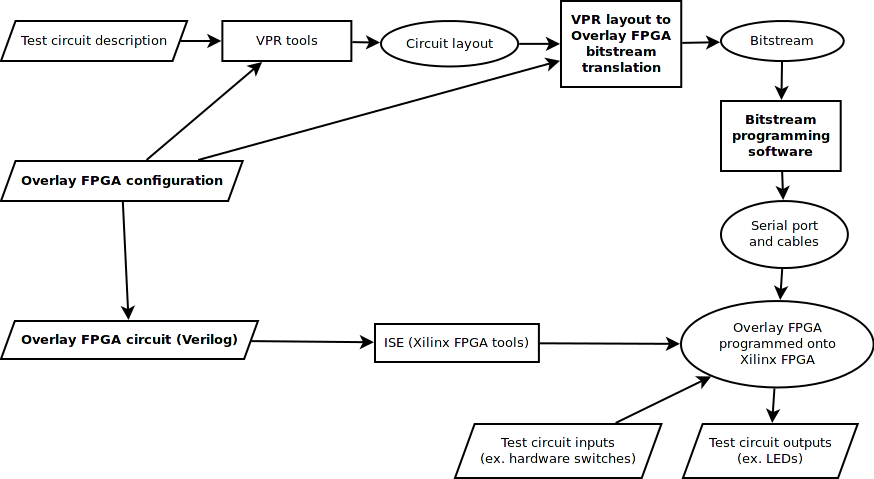
\includegraphics[scale=0.5]{system.png}
	\caption{System diagram}
	\label{system-diagram}
\end{figure}

The \emph{Overlay FPGA configuration} refers to the arrangement, size and connectivity of the logic blocks in the overlay FPGA circuit we are creating.
It appears in the Verilog as parameters, and is also used as configuration options in VPR and our bitstream translation tool.

The \emph{Overlay FPGA circuit} is a Verilog HDL circuit model of an FPGA which we will implement on a physical Xilinx FPGA.
In order to implement the circuit, we will run synthesis, placement and routing, then program it to the Xilinx FPGA using the ISE tools.
The end product will be the \emph{Overlay FPGA} implemented on a Xilinx Virtex 5 FPGA, shown in the lower right of \figref{system-diagram}.

In order to program a test circuit onto the Overlay FPGA, we will start by generating the test circuit layout using the \emph{VPR tools}.
This creates a circuit layout that is appropriate for our Overlay FPGA from the test circuit description.
We must then translate the circuit from VPR's format into a bitstream that can be programmed directly onto the Overlay FPGA.
Finally, the bitstream corresponding to the test circuit is programmed onto the Overlay FPGA.
The test circuit will be tested by using switches on the Xilinx FPGA development board as inputs, and LEDs on the board as outputs.



\subsection{Module-level descriptions} % for final proposal

\figref{module-diagram} shows the interactions between the modules we are designing.
The design consists of a software component that communicates with a hardware component through a serial interface.
The software components and implementation of the hardware component are described in \sectref{system-overview}.
This section focuses on the interactions between the hardware modules.

\begin{figure}[!h]
	\centering
	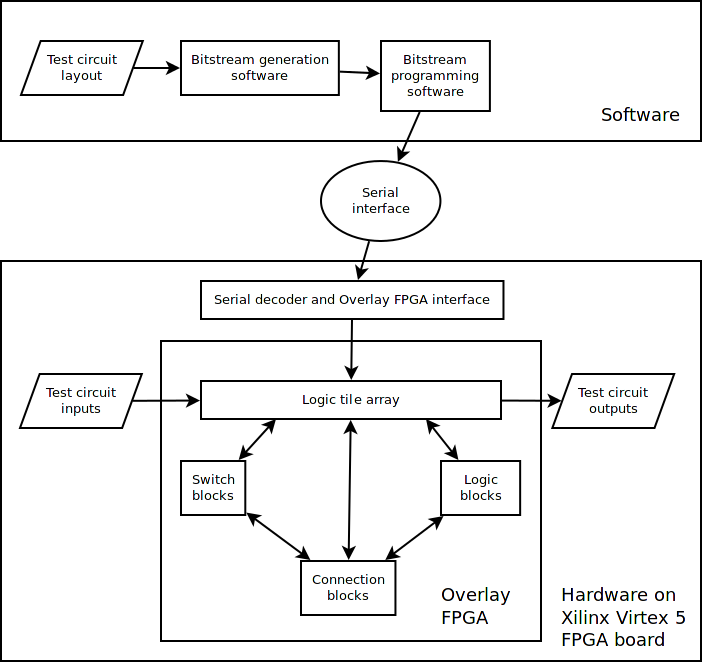
\includegraphics[scale=0.5]{modules.png}
	\caption{Module interaction}
	\label{module-diagram}
\end{figure}

The hardware components are all implemented on a Xilinx FPGA.
The hardware connects inputs and outputs to the \emph{Overlay FPGA}.
It also provides a serial decoder interface which is used to program a bitstream sent from the software component onto the Overlay FPGA.

The \emph{Overlay FPGA} consists of a two-dimensional array of \emph{tiles}.
The \emph{tiles} contain \emph{logic blocks}, \emph{switch blocks} and \emph{connection blocks}.
A \emph{logic block} contains the basic logic elements and wires to hook them up locally.
The \emph{connection blocks} connect logic blocks to switch blocks, and the \emph{switch blocks} connect connection blocks to other connection blocks, allowing global routing between logic blocks around the Overlay FPGA.


